%%
%% This is file `sample-sigconf.tex',
%% generated with the docstrip utility.
%%
%% The original source files were:
%%
%% samples.dtx  (with options: `sigconf')
%% 
%% IMPORTANT NOTICE:
%% 
%% For the copyright see the source file.
%% 
%% Any modified versions of this file must be renamed
%% with new filenames distinct from sample-sigconf.tex.
%% 
%% For distribution of the original source see the terms
%% for copying and modification in the file samples.dtx.
%% 
%% This generated file may be distributed as long as the
%% original source files, as listed above, are part of the
%% same distribution. (The sources need not necessarily be
%% in the same archive or directory.)
%%
%% The first command in your LaTeX source must be the \documentclass command.
\documentclass[sigconf]{acmart}

%%
%% \BibTeX command to typeset BibTeX logo in the docs
\AtBeginDocument{%
  \providecommand\BibTeX{{%
    \normalfont B\kern-0.5em{\scshape i\kern-0.25em b}\kern-0.8em\TeX}}}

%% Rights management information.  This information is sent to you
%% when you complete the rights form.  These commands have SAMPLE
%% values in them; it is your responsibility as an author to replace
%% the commands and values with those provided to you when you
%% complete the rights form.
\setcopyright{acmcopyright}
\copyrightyear{2018}
\acmYear{2018}
\acmDOI{10.1145/1122445.1122456}

%% These commands are for a PROCEEDINGS abstract or paper.
\acmConference[Woodstock '18]{Woodstock '18: ACM International Conference of Human-Robot Interaction}{8 March 2021}{Online}
\acmBooktitle{Woodstock '18: ACM International Conference of Human-Robot Interaction,
8 March 2021, Online}
\acmPrice{15.00}
\acmISBN{978-1-4503-XXXX-X/18/06}

\graphicspath{{../figures}} %goes to path: figures/

%%
%% Submission ID.
%% Use this when submitting an article to a sponsored event. You'll
%% receive a unique submission ID from the organizers
%% of the event, and this ID should be used as the parameter to this command.
%%\acmSubmissionID{123-A56-BU3}

%%
%% The majority of ACM publications use numbered citations and
%% references.  The command \citestyle{authoryear} switches to the
%% "author year" style.
%%
%% If you are preparing content for an event
%% sponsored by ACM SIGGRAPH, you must use the "author year" style of
%% citations and references.
%% Uncommenting
%% the next command will enable that style.
%%\citestyle{acmauthoryear}

%%
%% end of the preamble, start of the body of the document source.
\begin{document}

%%
%% The "title" command has an optional parameter,
%% allowing the author to define a "short title" to be used in page headers.
\title{AIR4children: Artificial Intelligence and Robotics for Children}
%%
%% The "author" command and its associated commands are used to define
%% the authors and their affiliations.
%% Of note is the shared affiliation of the first two authors, and the
%% "authornote" and "authornotemark" commands
%% used to denote shared contribution to the research.

%\author{Ben Trovato}
%\authornote{Both authors contributed equally to this research.}
%\email{trovato@corporation.com}
%\orcid{1234-5678-9012}
%\author{G.K.M. Tobin}

\author{Co-author A}
\affiliation{%
  \institution{University of A}
  \streetaddress{Adress}
  \city{City}
  \country{Country}}
\email{email@internet.org}

\author{Co-author B}
\affiliation{%
\institution{University of B}
\streetaddress{Adress}
\city{City}
\country{Country}}
\email{email@internet.org}

\author{Co-author C}
\affiliation{%
  \institution{University}
  \city{City}
  \country{Country}}
\authornotemark[1]
\email{e@mail.com}

%%
%% By default, the full list of authors will be used in the page
%% headers. Often, this list is too long, and will overlap
%% other information printed in the page headers. This command allows
%% the author to define a more concise list
%% of authors' names for this purpose.
\renewcommand{\shortauthors}{Lastname et al.}

%%
%% The abstract is a short summary of the work to be presented in the
%% article.
\begin{abstract}
  In this work, we proposed air4children, artificial intelligence for children as a way to both (a) tackle aspect for inclusion and non-discrimination, agency, privacy, dignity, transparency, equity, fairness and participation and (b) child-centre approach for AI and robotics.
  We introduce the present current challenges and opportunities for a child-centre approach for AI and robotics. 
  Similarly, we touch on open-sourced software and hardware technologigies to make a more inclusive, transparent and fair participation of children in areas of AIR. 
  Then, we describe the avenues that air4children can work with as development of open-sourced software and hardware, open-sourced teaching material. 
  Finally, we add conclusions and future work. 
\end{abstract}

%%
%% The code below is generated by the tool at http://dl.acm.org/ccs.cfm.
%% Please copy and paste the code instead of the example below.
%%
\begin{CCSXML}
<ccs2012>
     <concept>
         <concept_id>10003120.10003121.10011748</concept_id>
         <concept_desc>Human-centered computing~Empirical studies in HCI</concept_desc>
         <concept_significance>500</concept_significance>
         </concept>
     <concept>
         <concept_id>10003120.10011738.10011776</concept_id>
         <concept_desc>Human-centered computing~Accessibility systems and tools</concept_desc>
         <concept_significance>500</concept_significance>
         </concept>
     <concept>
         <concept_id>10010405.10010489.10010491</concept_id>
         <concept_desc>Applied computing~Interactive learning environments</concept_desc>
         <concept_significance>300</concept_significance>
         </concept>
     <concept>
         <concept_id>10003456.10010927.10010930.10010931</concept_id>
         <concept_desc>Social and professional topics~Children</concept_desc>
         <concept_significance>500</concept_significance>
         </concept>
     <concept>
         <concept_id>10010147.10010178.10010187.10010194</concept_id>
         <concept_desc>Computing methodologies~Cognitive robotics</concept_desc>
         <concept_significance>300</concept_significance>
         </concept>
</ccs2012>
\end{CCSXML}

\ccsdesc[500]{Human-centered computing~Empirical studies in HCI}
\ccsdesc[500]{Human-centered computing~Accessibility systems and tools}
\ccsdesc[300]{Applied computing~Interactive learning environments}
\ccsdesc[500]{Social and professional topics~Children}
\ccsdesc[300]{Computing methodologies~Cognitive robotics}

%%
%% Keywords. The author(s) should pick words that accurately describe
%% the work being presented. Separate the keywords with commas.
\keywords{Child-centred AI, Educational Robotics, Child-robot interaction}

%% A "teaser" image appears between the author and affiliation
%% information and the body of the document, and typically spans the
%% page.
\begin{teaserfigure}
  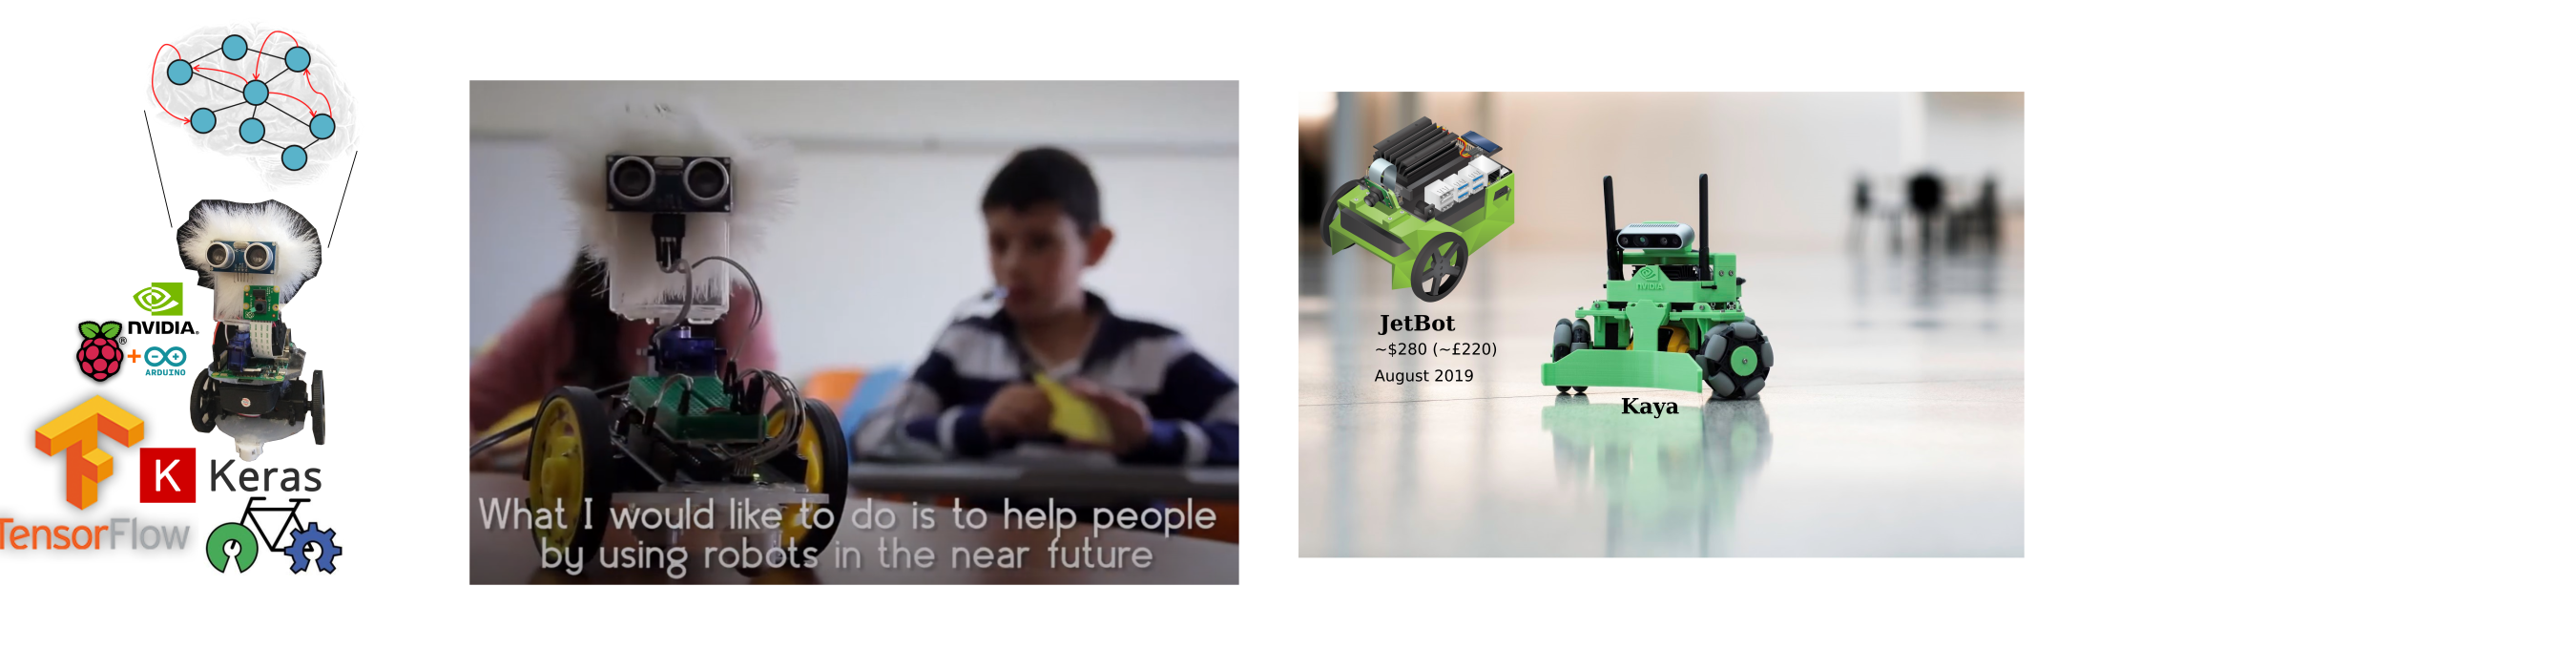
\includegraphics[width=\textwidth]{../figures/air4children/versions/drawing-v00.png}
  \caption{(a)open-source software and hardware, (b) non-traditional curriculums, (c) free for anyone.}
  \Description{Enjoying the baseball game from the third-base seats. Ichiro Suzuki preparing to bat.}
  \label{fig:teaser}
\end{teaserfigure}

%%
%% This command processes the author and affiliation and title
%% information and builds the first part of the formatted document.
\maketitle

\section{Introduction} 
The scientific and techonlogical progress in the fields of Artificial Intelligence and Robotics (AIR) is rapdily moving forward over the past decade. 
Advances in AIR are mainly in countries such as United States, China and Europe where support of such fields is part of their agenda \cite{Savage2020}. 
As the fielfs of AIR are advancing at a great pace, there are opportunties to for more child-centered AIR and with various challenges for children in places where resources are scarse. 
Recently, a drafted guidance of AI for children by UNICEF \cite{UNICEF2020} pointed out various challenges of making such filed avaiable to under-represented communities with the aim of providing fairness and non-discrimination.
With this in mind this work is proposing Artificial Intelligence and Robotics for Children (AIR4children) as a way to create and to design tools based on open-sourced projects.
Similarly, AIR4children is aiming to design curriculums with an non-traditional education approach for children of different socieconomical backgrounds, developmental stages or learning abilitities. 
%Anoother aspects as the socialbitly of robots are well explamplied with 
%Jibo [REF], Cosmos [REF] and more recently Shelly, a tortoise-like robot, to tacke 
%multiple interaction of one-to-many as well the resctrition of children
%abusive behaviours towards robots \cite{hu2018}. 

\section{Open Source AI and Robotics}
The spirit of open source software since 19XX with the contributions 
of users of different skills made a culture of openly share code to make
more robust tools (i.e. firefox, ubuntu, etc). Much recently, something 
similar to software is happening for hardware. One example is the community 
for arduino that open-sourced diagrams, code and with a low-cost microcontroller
magaged to make wordwile impact. See ~\ref{tab:opensourceprojects}.

This document will explain the major features of the document
class. For further information, the {\itshape \LaTeX\ User's Guide} is
available from
\url{https://www.acm.org/publications/proceedings-template}.


\subsection{Open Source AI}
[Section to describe open-source AI projects and related them to air4children].
As noted in the introduction, the ``\verb|acmart|'' document class can
be used to prepare many different kinds of documentation --- a
double-blind initial submission of a full-length technical paper, a
two-page SIGGRAPH Emerging Technologies abstract, a ``camera-ready''
journal article, a SIGCHI Extended Abstract, and more --- all by
selecting the appropriate {\itshape template style} and {\itshape
  template parameters}.

  Deep Learning (DL) is a branch of machine learning in Artificial Intelligence
  which essentially takes advantage of a huge datasets to train neural networks.
  The great impact of DL in recent years is also because of improvements in 
  hardware development and mainly because of open source tools and libraries \cite{matelabs2017}.
  Additionally to that, there is a huge range of applications in areas such as robotics,
  transportation, medicine and last but not least in education.
  That said, we propose to use a raspberry pi, a $\pounds$30 board with
  GNU/Linux OS, connected with a mini arduino board, $\pounds$2 board,  servomotors 
  and pi camera in order to create a simple low-cost educational robot 
  where children can learn the basics concepts of robotics and deep learning \cite{durr2015}.
  
    

\subsection{Open Source Robotics}
[Section to describe open-source robotics projects and related them to air4children.]
As noted in the introduction, the ``\verb|acmart|'' document class can
be used to prepare many different kinds of documentation --- a
double-blind initial submission of a full-length technical paper, a
two-page SIGGRAPH Emerging Technologies abstract, a ``camera-ready''
journal article, a SIGCHI Extended Abstract, and more --- all by
selecting the appropriate {\itshape template style} and {\itshape
  template parameters}.

\section{Open AIR4Children}
[Section to describe the proposed project of air4children and the integration 
of opensource tools.]
The ``\verb|acmart|'' document class includes the ``\verb|booktabs|''
package --- \url{https://ctan.org/pkg/booktabs} --- for preparing
high-quality tables.

Table captions are placed {\itshape above} the table.

Because tables cannot be split across pages, the best placement for
them is typically the top of the page nearest their initial cite.  To
ensure this proper ``floating'' placement of tables, use the
environment \textbf{table} to enclose the table's contents and the
table caption.  The contents of the table itself must go in the
\textbf{tabular} environment, to be aligned properly in rows and
columns, with the desired horizontal and vertical rules.  Again,
detailed instructions on \textbf{tabular} material are found in the
\textit{\LaTeX\ User's Guide}.

Immediately following this sentence is the point at which
Table~\ref{tab:freq} is included in the input file; compare the
placement of the table here with the table in the printed output of
this document.

\begin{table}
  \caption{Open source projects}
  \label{tab:opensourceprojects}
  \begin{tabular}{ccl}
    \toprule
    Project name& Year of creation & Community\\
    \midrule
    JetBot AI Robot \cite{nanoJetBot:2019} & March 2019 & - \\
    JPL Open Source Rover \cite{OSR:2018} & April 2018 & - \\
    Otto DIY robots \cite{OttoDIY:2016} & 2016 & 50K used robots in >70 countries\\
    $\Psi^2_1$ & 1 in 40,000& Unexplained usage\\
  \bottomrule
\end{tabular}
\end{table}


\subsection{Open hardware and software}
[Section to describe the hardware and software that can be used in 
air4children.]
The ``\verb|figure|'' environment should be used for figures. One or
more images can be placed within a figure. If your figure contains
third-party material, you must clearly identify it as such, as shown
in the example below.
\begin{figure}[h]
  \centering
  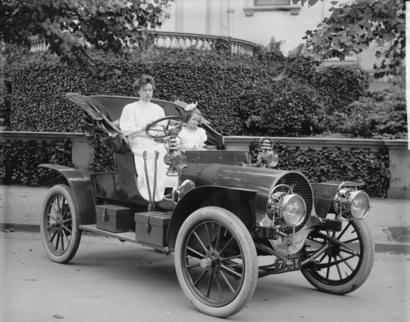
\includegraphics[width=\linewidth]{sample-franklin}
  \caption{1907 Franklin Model D roadster. Photograph by Harris \&
    Ewing, Inc. [Public domain], via Wikimedia
    Commons. (\url{https://goo.gl/VLCRBB}).}
  \Description{A woman and a girl in white dresses sit in an open car.}
\end{figure}

Your figures should contain a caption which describes the figure to
the reader.

Figure captions are placed {\itshape below} the figure.

Every figure should also have a figure description unless it is purely
decorative. These descriptions convey what’s in the image to someone
who cannot see it. They are also used by search engine crawlers for
indexing images, and when images cannot be loaded.

A figure description must be unformatted plain text less than 2000
characters long (including spaces).  {\bfseries Figure descriptions
  should not repeat the figure caption – their purpose is to capture
  important information that is not already provided in the caption or
  the main text of the paper.} For figures that convey important and
complex new information, a short text description may not be
adequate. More complex alternative descriptions can be placed in an
appendix and referenced in a short figure description. For example,
provide a data table capturing the information in a bar chart, or a
structured list representing a graph.  For additional information
regarding how best to write figure descriptions and why doing this is
so important, please see
\url{https://www.acm.org/publications/taps/describing-figures/}.

Our primary aim for Libre Robotics is to build low-cost education robots 
which will be helpful to teach many didactic activities where children 
can interact with the robot and learn concepts of robotics, linear algebra, 
machine learning, and deep learning.
One example is the implementation of a low-cost robot with 
convolutional neural networks that recognise six basic face emotions: 
happy, sad, surprise, fear, anger and neutral \cite{ho2016, Ruiz-Garcia2016}. 

\subsection{Open teaching materials}
Considering the work of Maria Montessori who emphasized “the hand is the instrument of the mind.” \cite{montessori2013absorbent}. 
That said, children must develop concentration to develop their learning skills. 
For instance, the best way a child can concentrate is by fixing his attention on some task he is performing with his hands. 
It is through movement and repetition that the child gets experience, allowing him to internalize new concepts. 
One potential way to develip such skills is the help of activities in engigering and robotics. 
Engineering and robotics has demonstrated that young children can experience a range of cognitive and social benefits when these materials are approprietely introduced in development stages [add berg2018, Bers-Horn, 2010; Kazakoff-Bers, 2012)].
Engineering tasks in robotics allow children to participate in creative explorations, develop fine motor skills and hand-eye coordination, engage in collaboration and teamwork \cite{elkin2014}.
Similarly, the children development of grasping and understanding mathematical concepts such as number, size, and shape (Bers, 2012; Resnick et al., 1998).

In that way, air4children's workshop integrates various hands-on activities where the children will develop different intellectual and social skills to incorporate into other areas of their lives.
More specifically, such workshops are based on several Montessori principles such as: moving from the simple to the complex, the concrete to the abstract, the familiar to the unfamiliar and the general to the specific, as well as a mixed age group, where children can learn from each other.
For instance, Elkin et al. (2014) \cite{elkin2014} explained how Robotics can also provide a way to engage children in problem-solving. 
Finding solutions together translate to social situations as well as it provides children with the foundations for decision making, logical reasoning, categorizing, analytical thinking, negotiation, and creativity. 
Children who think creatively are curious and open-minded, have a sense of wonder and joy in learning.

Using a variety of teaching materials that combine theory and practice, our workshop has the goal to create experiences to build children’s confidence, develop creativity, teamwork and curiosity.

%[Section to describe open teaching materials, perhaps using non-traditional education systems.]
%Serholt 2017 performed studies to quantify the social intereaction 
%between robots and children (i.e., gaze, verbal interaction, gestures, 
%and facial expressions). However robotics tutors are not yet to the point 
%to deal with complex child-robot interactions. 
%\cite{Serholt:2017}

\section{Conclusions and future work}
[for conclusions and future work].
The use of \BibTeX\ for the preparation and formatting of one's
references is strongly recommended. Authors' names should be complete
--- use full first names (``Donald E. Knuth'') not initials
(``D. E. Knuth'') --- and the salient identifying features of a
reference should be included: title, year, volume, number, pages,
article DOI, etc.
A ``teaser figure'' is an image, or set of images in one figure, that
are placed after all author and affiliation information, and before
the body of the article, spanning the page. If you wish to have such a
figure in your article, place the command immediately before the
\verb|\maketitle| command:
\begin{verbatim}
  \begin{teaserfigure}
    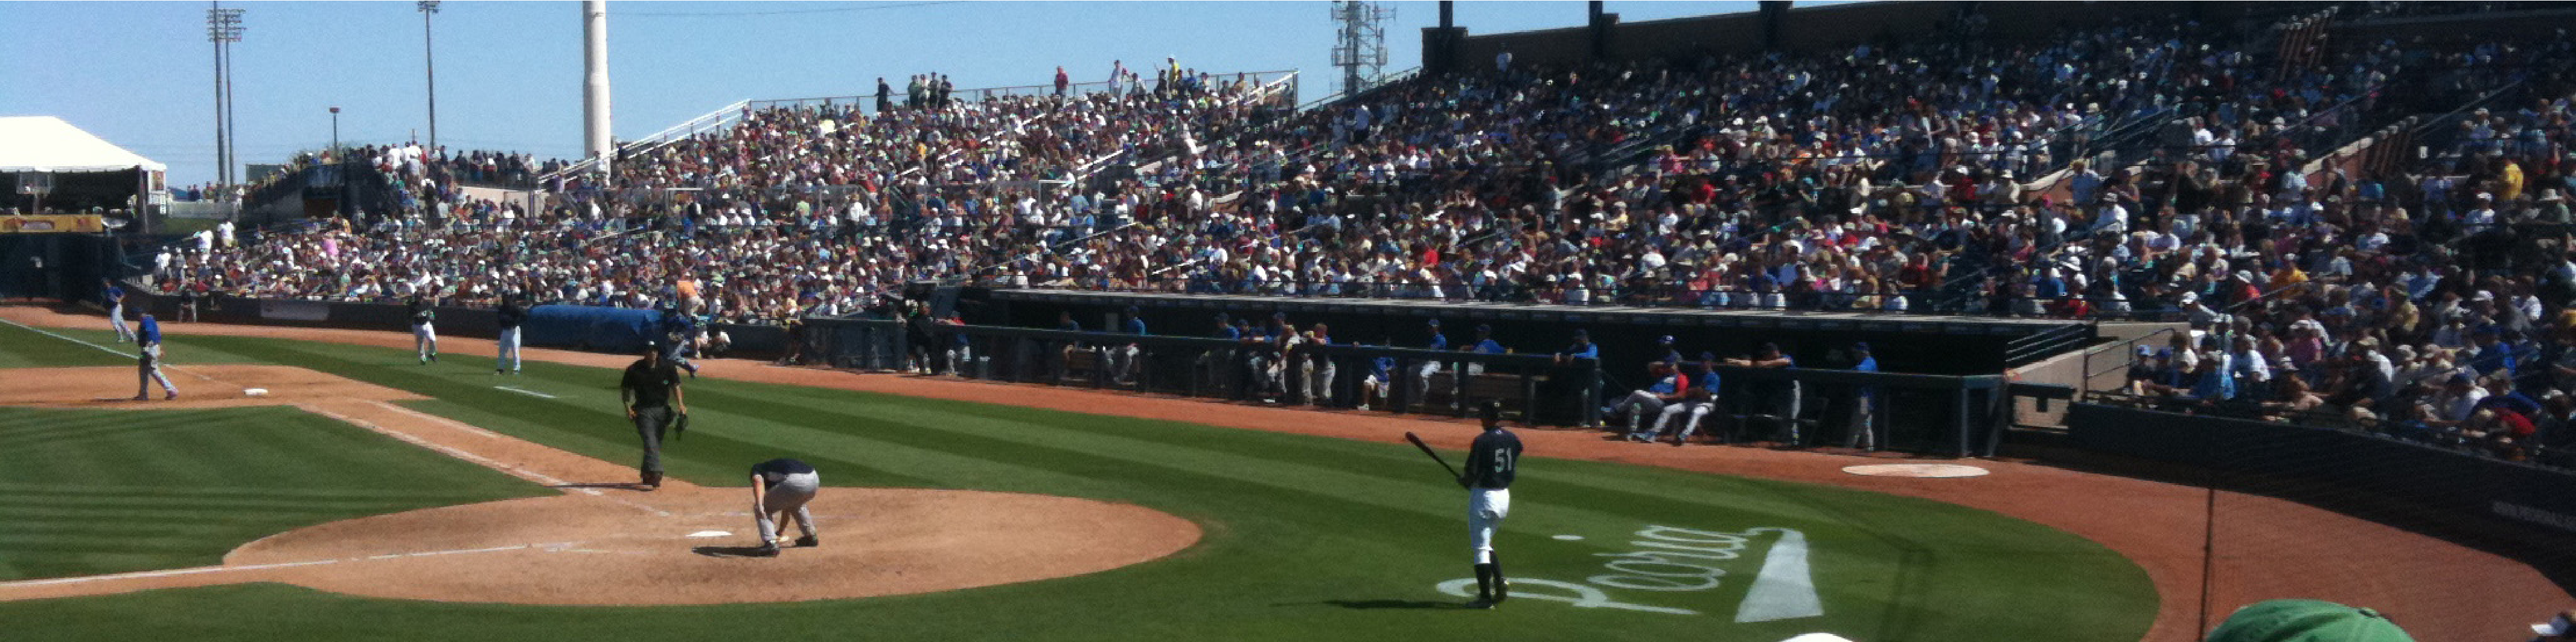
\includegraphics[width=\textwidth]{sampleteaser}
    \caption{figure caption}
    \Description{figure description}
  \end{teaserfigure}
\end{verbatim}


The bibliography is included in your source document with these two
commands, placed just before the \verb|\end{document}| command:
\begin{verbatim}
  \bibliographystyle{ACM-Reference-Format}
  \bibliography{bibfile}
\end{verbatim}
where ``\verb|bibfile|'' is the name, without the ``\verb|.bib|''
suffix, of the \BibTeX\ file.

Citations and references are numbered by default. A small number of
ACM publications have citations and references formatted in the
``author year'' style; for these exceptions, please include this
command in the {\bfseries preamble} (before the command
``\verb|\begin{document}|'') of your \LaTeX\ source:
\begin{verbatim}
  \citestyle{acmauthoryear}
\end{verbatim}

  Some examples.  A paginated journal article \cite{UNICEF2020}
  %, an
  %enumerated journal article \cite{Cohen07}, a reference to an entire
  %issue \cite{JCohen96}, a monograph (whole book) \cite{Kosiur01}, a
  %monograph/whole book in a series (see 2a in spec. document).
  %tech report: \cite{Harel78},
  %online: \cite{Thornburg01},
  %online: \cite{Ablamowicz07},
  %misc: \cite{Poker06}
  %misc: \cite{Obama08}
  %manuals:  \cite{Fear05},
  % \cite{Amsthm15}

%  \cite{Harel79}, a divisible-book such as an anthology or compilation
%  \cite{Editor00} followed by the same example, however we only output
%  the series if the volume number is given \cite{Editor00a} (so
%  Editor00a's series should NOT be present since it has no vol. no.),
%  a chapter in a divisible book \cite{Spector90}, a chapter in a
%  divisible book in a series \cite{Douglass98}, a multi-volume work as
%  book \cite{Knuth97}, a couple of articles in a proceedings (of a
%  conference, symposium, workshop for example) (paginated proceedings
%  article) \cite{Andler79, Hagerup1993}, a proceedings article with
%  all possible elements \cite{Smith10}, an example of an enumerated
%  proceedings article \cite{VanGundy07}, an informally published work
%  \cite{Harel78}, a couple of preprints \cite{Bornmann2019,
%    AnzarootPBM14}, a doctoral dissertation \cite{Clarkson85}, a
%  master's thesis: \cite{anisi03}, an online document / world wide web
% resource \cite{Thornburg01, Ablamowicz07, Poker06}, a video game
%  (Case 1) \cite{Obama08} and (Case 2) \cite{Novak03} and \cite{Lee05}
%  and (Case 3) a patent \cite{JoeScientist001}, work accepted for
%  publication \cite{rous08}, 'YYYYb'-test for prolific author
%  \cite{SaeediMEJ10} and \cite{SaeediJETC10}. Other cites might
%  contain 'duplicate' DOI and URLs (some SIAM articles)
%  \cite{Kirschmer:2010:AEI:1958016.1958018}. Boris / Barbara Beeton:
%  multi-volume works as books \cite{MR781536} and \cite{MR781537}. A
%  couple of citations with DOIs:
%  \cite{2004:ITE:1009386.1010128,Kirschmer:2010:AEI:1958016.1958018}. Online
%  citations: \cite{TUGInstmem, Thornburg01, CTANacmart}. Artifacts:
%  \cite{R} and \cite{UMassCitations}.

%%
%% The acknowledgments section is defined using the "acks" environment
%% (and NOT an unnumbered section). This ensures the proper
%% identification of the section in the article metadata, and the
%% consistent spelling of the heading.
\begin{acks}
To Robert, for the bagels and explaining CMYK and color spaces.
\end{acks}

%%
%% The next two lines define the bibliography style to be used, and
%% the bibliography file.
\bibliographystyle{ACM-Reference-Format}
\bibliography{../references/references}


\end{document}
\endinput
%%
%% End of file `sample-sigconf.tex'.
